%!TEX program = xelatex
\documentclass[11pt, a4paper]{article}

% AA LINGUA E GESTIONE FONT (Specifica per XeLaTeX)
\usepackage{fontspec}
\setmainfont{Latin Modern Roman}
\usepackage[italian]{babel}

% AA LAYOUT DI PAGINA E TIPOGRAFIA (Ottimizzato per Rilegatura)
\usepackage[left=2.4cm, right=1.6cm, top=2cm, bottom=2cm]{geometry}

% AA Spaziatura tra paragrafi controllata (compatta ed evita salti enormi)
\usepackage[skip=3pt plus 1pt minus 1pt]{parskip}
\setlength{\parindent}{0pt}

% AA Microtype per XeLaTeX
\usepackage[protrusion=true]{microtype}
\raggedbottom

% AA GESTIONE DEI COLORI
\usepackage{xcolor}

% AA MATEMATICA E SIMBOLI
\usepackage{amsmath}
\usepackage{mathtools}
\usepackage{silence}
\usepackage[warnings-off={mathtools-overbracket,mathtools-colon}]{unicode-math}
\setmathfont{Latin Modern Math}

% BB OTTIMIZZAZIONE MATRICI LUNGHE PER LA STAMPA
\setlength{\arraycolsep}{10pt}

% AA Spaziature verticali attorno alle formule matematiche
\setlength{\abovedisplayskip}{3pt plus 1pt minus 1pt}
\setlength{\belowdisplayskip}{3pt plus 1pt minus 1pt}
\setlength{\abovedisplayshortskip}{0pt plus 1pt}
\setlength{\belowdisplayshortskip}{2pt plus 1pt minus 1pt}

% AA GRAFICA ED IMMAGINI
\usepackage{graphicx}
\graphicspath{{./E3_1_Images/}}

% AA PERSONALIZZAZIONE TITOLI
\usepackage{titlesec}
\titleformat{\section}{\normalfont\Large\bfseries\color{blue!80!black}}{\thesection}{1em}{}
\titleformat{name=\section,numberless}{\normalfont\Large\bfseries\color{blue!80!black}}{}{0pt}{}

\titleformat{\subsection}{\normalfont\large\bfseries}{\thesubsection}{1em}{}
\titleformat{name=\subsection,numberless}{\normalfont\large\bfseries}{}{0pt}{}

\titleformat{\subsubsection}{\normalfont\normalsize\bfseries}{\thesubsubsection}{1em}{}
\titleformat{name=\subsubsection,numberless}{\normalfont\normalsize\bfseries}{}{0pt}{}

\titlespacing*{\section}{0pt}{1.2ex plus 0.4ex minus 0.2ex}{0.6ex plus 0.2ex}
\titlespacing*{\subsection}{0pt}{1ex plus 0.3ex minus 0.2ex}{0.5ex plus 0.2ex}
\titlespacing*{\subsubsection}{0pt}{0.8ex plus 0.2ex minus 0.1ex}{0.4ex plus 0.1ex}

\titleformat{\paragraph}[block]{\normalfont\normalsize\bfseries\color{black!80!black}\raggedright}{}{0pt}{}
\titlespacing*{\paragraph}{0pt}{1.2ex plus 0.3ex minus 0.2ex}{0.4ex}

% AA INTEGRAZIONE CODICE MATLAB
\usepackage{matlab}

% BB Riconfigurazione Automatica Titoli Esportati da MATLAB
\renewcommand{\matlabheading}[1]{\section*{#1}}
\renewcommand{\matlabheadingtwo}[1]{\subsection*{#1}}
\renewcommand{\matlabheadingthree}[1]{\subsubsection*{#1}}

% BB Formule E Matrici Simboliche
\renewenvironment{matlabsymbolicoutput}{%
  \par\vspace{2pt}%
  \begingroup
  \centering
}{%
  \par\vspace{2pt}%
  \endgroup
}

% BB Output Testuale Console
\renewenvironment{matlaboutput}{%
  \par\vspace{1pt}%
  \Verbatim[xleftmargin=10pt, formatcom=\color{black!75}, fontsize=\footnotesize]%
}{%
  \endVerbatim
  \vspace{1pt}%
}

% BB Box Codice (Stile Moderno con Barra Laterale Colorata)
\lstset{
  backgroundcolor={},
  aboveskip=0pt,
  belowskip=0pt,
  basicstyle=\ttfamily\footnotesize,
  xleftmargin=0pt
}

\mdfdefinestyle{matlabcode}{%
  topline=false,
  bottomline=false,
  rightline=false,
  leftline=true,
  linewidth=2.5pt,
  linecolor=blue!75!black,
  backgroundcolor=black!3,
  innertopmargin=4pt,
  innerbottommargin=4pt,
  innerleftmargin=9pt,
  innerrightmargin=6pt,
  skipabove=3pt,
  skipbelow=3pt
}

\allowdisplaybreaks

% AA LINK, METADATI ED ELENCHI
\usepackage{hyperref}
\hypersetup{
    colorlinks=true,
    linkcolor=blue!80!black,
    urlcolor=blue!80!black,
    citecolor=blue!80!black,
    pdftitle={Cinematica Diretta Manipolatore Sferico Tipo I},
    pdfauthor={Francesco Lo Verde},
}
\usepackage{bookmark}

% BB Spaziatura Elenchi (Arieggiata per la Stampa)
\usepackage{enumitem}
\setlist{itemsep=3.5pt plus 1pt minus 1pt, topsep=4pt plus 1pt minus 1pt, partopsep=0pt, parsep=1pt}


\author{Francesco Lo Verde}
\begin{document}

\matlabtitle{Calcolo Cinematica Diretta Con Parametri Di Denavit-Hartenberg}

\begin{par}
\begin{flushleft}
L'obiettivo della cinematica diretta è determinare la posizione e l'orientamento dell'organo terminale (end-effector) a partire dai valori delle variabili di giunto. Si utilizza la convenzione di Denavit-Hartenberg (DH) per modellare la geometria del robot. La convenzione di Denavit-Hartenberg è un metodo standard per assegnare sistemi di riferimento ai bracci di un robot. Per ogni braccio, si definiscono quattro parametri che descrivono la trasformazione geometrica rispetto al braccio precedente.
\end{flushleft}
\end{par}

\begin{par}
\begin{flushleft}
Si inizia definendo le variabili simboliche necessarie per i parametri DH. Questo permette di eseguire i calcoli in forma generale, senza dover specificare subito valori numerici. Successivamente, si assemblano questi parametri in una tabella dove ogni riga corrisponde a un giunto del robot e le colonne rappresentano i parametri $\left(\begin{array}{c}
\theta ,d,\alpha ,a
\end{array}\right)$.
\end{flushleft}
\end{par}

\begin{matlabcode}
clc; clear; close all;

% Definizione Variabili Simboliche
syms q1 q2 q3 real;
syms d0 d1 a3 real;

DH_table = [q1, d0, -pi/2, d1;
            q2, 0,  -pi/2, 0;
            q3, 0,  0,     a3];

% Numero Giunti Manipolatore
n = size(DH_table, 1);
\end{matlabcode}

\begin{par}
\begin{flushleft}
A partire dalla tabella DH, si può calcolare la matrice di trasformazione omogenea $A_i$ per ciascun giunto $i$. Questa matrice, di dimensioni $4\times 4$ e rappresenta la trasformazione (rotazione e traslazione) dal sistema di riferimento del giunto $i$ a quello del giunto $i-1$. Si utilizza la funzione \texttt{Compute\_DH\_Transformations }per generare le matrici simboliche per ogni riga della tabella DH.
\end{flushleft}
\end{par}

\begin{matlabcode}
% Calcolo Matrici Trasformazione
[T_matrices, R_matrices] = Compute_DH_Transformations(DH_table);

% Visualizzazione Matrici Trasformazione
for i = 1:n
    fprintf('Matrice Di Trasformazione Omogenea A%d:\n', i);
    disp(T_matrices(:,:,i));
end
\end{matlabcode}
\begin{matlaboutput}
Matrice Di Trasformazione Omogenea A1:
\end{matlaboutput}
\begin{matlabsymbolicoutput}
\hskip1em $\displaystyle \left(\begin{array}{cccc}
\cos \left(q_1 \right) & 0 & -\sin \left(q_1 \right) & d_1 \,\cos \left(q_1 \right)\\
\sin \left(q_1 \right) & 0 & \cos \left(q_1 \right) & d_1 \,\sin \left(q_1 \right)\\
0 & -1 & 0 & d_0 \\
0 & 0 & 0 & 1
\end{array}\right)$
\end{matlabsymbolicoutput}
\begin{matlaboutput}
Matrice Di Trasformazione Omogenea A2:
\end{matlaboutput}
\begin{matlabsymbolicoutput}
\hskip1em $\displaystyle \left(\begin{array}{cccc}
\cos \left(q_2 \right) & 0 & -\sin \left(q_2 \right) & 0\\
\sin \left(q_2 \right) & 0 & \cos \left(q_2 \right) & 0\\
0 & -1 & 0 & 0\\
0 & 0 & 0 & 1
\end{array}\right)$
\end{matlabsymbolicoutput}
\newpage
\begin{matlaboutput}
Matrice Di Trasformazione Omogenea A3:
\end{matlaboutput}
\begin{matlabsymbolicoutput}
\hskip1em $\displaystyle \left(\begin{array}{cccc}
\cos \left(q_3 \right) & -\sin \left(q_3 \right) & 0 & a_3 \,\cos \left(q_3 \right)\\
\sin \left(q_3 \right) & \cos \left(q_3 \right) & 0 & a_3 \,\sin \left(q_3 \right)\\
0 & 0 & 1 & 0\\
0 & 0 & 0 & 1
\end{array}\right)$
\end{matlabsymbolicoutput}

\begin{par}
\begin{flushleft}
Per ottenere la posa dell'organo terminale rispetto alla base del robot, si moltiplicano in sequenza le matrici di trasformazione individuali. Il risultato è la matrice di trasformazione omogenea totale $^0 T_n$, che contiene sia la matrice di rotazione $^0 R_n$ (orientamento) sia il vettore di posizione $^0 p_n$ dell'end-effector.
\end{flushleft}
\end{par}

\begin{par}
$$^0 T_n =A_1 \cdot A_2 \cdot \ldots\cdot A_n$$
\end{par}

\begin{matlabcode}
% Calcolo Matrice Di Trasformazione Totale Dalla Base All'End Effector
T0n = T_matrices(:,:,1) * T_matrices(:,:,2) * T_matrices(:,:,3);
T0n = simplify(T0n);

fprintf('Matrice Di Trasformazione Omogenea Totale T03:\n');
disp(T0n);
\end{matlabcode}
\begin{matlaboutput}
Matrice Di Trasformazione Omogenea Totale T03:
\end{matlaboutput}
\resizebox{\linewidth}{!}{%
$
    \begin{pmatrix}
        s\left(q_1 \right)\,s\left(q_3 \right)+c\left(q_1 \right)\,c\left(q_2 \right)\,c\left(q_3 \right) & c\left(q_3 \right)\,s\left(q_1 \right)-c\left(q_1 \right)\,c\left(q_2 \right)\,s\left(q_3 \right) & -c\left(q_1 \right)\,s\left(q_2 \right) & d_1 \,c\left(q_1 \right)+a_3 \,s\left(q_1 \right)\,s\left(q_3 \right)+a_3 \,c\left(q_1 \right)\,c\left(q_2 \right)\,c\left(q_3 \right)\\
        c\left(q_2 \right)\,c\left(q_3 \right)\,s\left(q_1 \right)-c\left(q_1 \right)\,s\left(q_3 \right) & -c\left(q_1 \right)\,c\left(q_3 \right)-c\left(q_2 \right)\,s\left(q_1 \right)\,s\left(q_3 \right) & -s\left(q_1 \right)\,s\left(q_2 \right) & d_1 \,s\left(q_1 \right)-a_3 \,c\left(q_1 \right)\,s\left(q_3 \right)+a_3 \,c\left(q_2 \right)\,c\left(q_3 \right)\,s\left(q_1 \right)\\
        -c\left(q_3 \right)\,s\left(q_2 \right) & s\left(q_2 \right)\,s\left(q_3 \right) & -c\left(q_2 \right) & d_0 -a_3 \,c\left(q_3 \right)\,s\left(q_2 \right)\\
        0 & 0 & 0 & 1
    \end{pmatrix}
$}
\begin{par}
\begin{flushleft}
Dalla matrice totale $^0 T_n$ si può estrarre la sottomatrice di rotazione $3\times 3$ e il vettore di posizione $3\times 1$
\end{flushleft}
\end{par}

\begin{matlabcode}
% Matrice Di Rotazione R03
R0n = T0n(1:3, 1:3);
R0n = simplify(R0n);
fprintf('Matrice Di Rotazione R03:\n');
disp(R0n);
\end{matlabcode}
\begin{matlaboutput}
Matrice Di Rotazione R03:
\end{matlaboutput}
\resizebox{\linewidth}{!}{%
$
\begin{pmatrix}
    s \left(q_1 \right)\,s \left(q_3 \right)+c\left(q_1 \right)\,c\left(q_2 \right)\,c\left(q_3 \right) & c\left(q_3 \right)\,s \left(q_1 \right)-c\left(q_1 \right)\,c\left(q_2 \right)\,s \left(q_3 \right) & -c\left(q_1 \right)\,s \left(q_2 \right)\\
    c\left(q_2 \right)\,c\left(q_3 \right)\,s \left(q_1 \right)-c\left(q_1 \right)\,s \left(q_3 \right) & -c\left(q_1 \right)\,c\left(q_3 \right)-c\left(q_2 \right)\,s \left(q_1 \right)\,s \left(q_3 \right) & -s \left(q_1 \right)\,s \left(q_2 \right)\\
    -c\left(q_3 \right)\,s \left(q_2 \right) & s \left(q_2 \right)\,s \left(q_3 \right) & -c\left(q_2 \right)
\end{pmatrix}
$}

\begin{matlabcode}
% Vettore Posizione p03
p0n = T0n(1:3, 4);
p0n = simplify(p0n);
fprintf('Vettore Posizione p03:\n');
disp(p0n);
\end{matlabcode}
\begin{matlaboutput}
Vettore Posizione p03:
\end{matlaboutput}
\begin{matlabsymbolicoutput}
\hskip1em $\displaystyle \left(\begin{array}{c}
d_1 \,\cos \left(q_1 \right)+a_3 \,\sin \left(q_1 \right)\,\sin \left(q_3 \right)+a_3 \,\cos \left(q_1 \right)\,\cos \left(q_2 \right)\,\cos \left(q_3 \right)\\
d_1 \,\sin \left(q_1 \right)-a_3 \,\cos \left(q_1 \right)\,\sin \left(q_3 \right)+a_3 \,\cos \left(q_2 \right)\,\cos \left(q_3 \right)\,\sin \left(q_1 \right)\\
d_0 -a_3 \,\cos \left(q_3 \right)\,\sin \left(q_2 \right)
\end{array}\right)$
\end{matlabsymbolicoutput}

\begin{par}
\newpage
\begin{flushleft}
Per visualizzare una configurazione specifica del robot sono necessari dei valori numerici. Si sostituiscono ora le variabili simboliche (angoli di giunto e parametri geometrici) con valori numerici.
\end{flushleft}
\end{par}

\begin{matlabcode}
% Lista Variabili Simboliche Da Sostituire
varsToSub = [q1, q2, q3, d0, d1, a3];

% Lista Valori Numerici Corrispondenti
% Esempio: q1=30°, q2=45°, q3=0°, d0=1, d1=0.5, a3=0.5
numValues = [pi/6, pi/4, 0, 1, 0.5, 0.5];

% Sostituzione Valori
T_Num = sym(zeros(4, 4, n));
for i = 1:n
    T_Num(:,:,i) = subs(T_matrices(:,:,i), varsToSub, numValues);
end

% Calcolo Matrice Numerica
T0n_Num = double(subs(T0n, varsToSub, numValues));
fprintf('Matrice Di Trasformazione Totale Numerica T03:\n');
disp(T0n_Num);
\end{matlabcode}
\begin{matlaboutput}
Matrice Di Trasformazione Totale Numerica T03:
\end{matlaboutput}
\begin{matlaboutput}
    0.6124    0.5000   -0.6124    0.7392
    0.3536   -0.8660   -0.3536    0.4268
   -0.7071         0   -0.7071    0.6464
         0         0         0    1.0000
\end{matlaboutput}

\matlabheading{Visualizzazione Grafica Manipolatore}

\begin{matlabcode}
figure;
hold on;
grid on;
xlabel('X');
ylabel('Y');
zlabel('Z');
axis equal;

% Definizione Colori Assi X, Y, Z (standard RGB)
colors = {'r', 'g', 'b'};
% Scala Per Le Frecce Degli Assi
arrow_scale = 0.2;
% Etichette
labels = {'Base', 'Giunto 1', 'Giunto 2', 'End-Effector'};

% T_cumulative Tiene Traccia Della Trasformazione Dalla Base Al Frame
% Corrente
T_cumulative = eye(4);
% Memorizza Posizioni Origini Frame
positions = T_cumulative(1:3, 4)';

% Frame Base
for j = 1:3
    quiver3(0, 0, 0, T_cumulative(1,j)*arrow_scale, T_cumulative(2,j)*arrow_scale, T_cumulative(3,j)*arrow_scale, ...
        'Color', colors{j}, 'LineWidth', 2, 'MaxHeadSize', 0.4);
end
text(0, 0, 0, [' ' labels{1}], 'FontSize', 10);
\end{matlabcode}
\newpage
\begin{matlabcode}
% Vettori Per Leggenda
h_axes = zeros(1, 3);

% Iterazione Giunti Per Ottenere Posa
for i = 1:n
    % Aggiorna Matrice Trasformazione Cumulativa
    T_cumulative = T_cumulative * double(T_Num(:,:,i));

    % Estrazione Posizione E Orientamento
    pos = T_cumulative(1:3, 4);
    R = T_cumulative(1:3, 1:3);

    % Assi Frame Corrente
    for j = 1:3
        h_axes(j) = quiver3(pos(1), pos(2), pos(3), R(1,j)*arrow_scale, R(2,j)*arrow_scale, R(3,j)*arrow_scale, ...
                             'Color', colors{j}, 'LineWidth', 2, 'MaxHeadSize', 0.4);
    end

    % Memorizza Pozione Corrente Per Disegnare Bracci
    positions = [positions; pos'];

    % Etichette
    text(pos(1), pos(2), pos(3), [' ' labels{i+1}], 'FontSize', 10);
end

% Disegna I Bracci
h_line = plot3(positions(:,1), positions(:,2), positions(:,3), 'k-o', 'LineWidth', 1.5, 'MarkerSize', 5, 'MarkerFaceColor', 'k');


legend([h_axes, h_line], {'Asse X', 'Asse Y', 'Asse Z', 'Bracci'}, 'Location', 'Best');
title('Configurazione Manipolatore Sferico Tipo I');
view(45, 25);
axis tight;
hold off;
\end{matlabcode}
\begin{center}
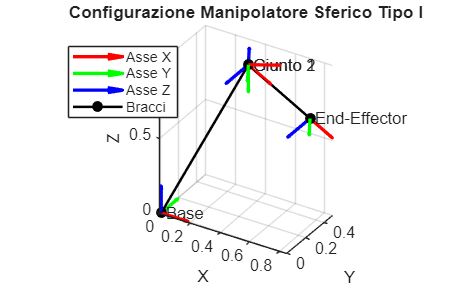
\includegraphics[width=0.8\linewidth]{figure_0.png}
\end{center}

\end{document}
